\documentclass[a4paper]{article}

\usepackage{listings}
\usepackage{graphicx}
\usepackage{float}
\usepackage[hidelinks]{hyperref}

%opening
\title{Deep Reinforcement Learning Tutorial \\Installation Guide}
\author{Julian Bernhardt, Robin Guth}

\begin{document}

\maketitle
\tableofcontents

\section{Introduction}
Deep Reinforcement Learning (also called RL) is a huge step towards the creation of an universal artificial intelligence.\\ %TODO ADD SOME SPICE
This guide will lead the reader through the setup process for the beginner tutorial "Deep Reinforcement Learning". 
\paragraph{Prerequisites}
It is recommended that a reader already acquired some basic knowledge about programming with Python and is familiar with basic deep learning concepts like Un-/Supervised Learning. It is also useful to be able to perform some basic linux commands, as we will use them later to install some additional packages.
\paragraph{Outlook}
The user will get to know basic concepts of RL with the help of:
\begin{description}
	\item[Python3] One of the most popular programming languages for deep learning. The following tutorials will be based on Python. See \url{https://www.python.org/} for more information.
	\item[Pip] A package installer for Python, which will download and install packages for us from a repository.
	\item[Jupyter Lab] Enables execution of Python code inside a document, used to teach theory and implementation. 
	\item[Google Cloud] Cloud based processing power for training of different implementations of RL. Delivers a linux environment with preinstalled utilities for deep learning including different libraries for Python, Python itself and Jupyter Lab.
\end{description}  
\section{Installation}
\subsection{Google Cloud}
As "Reinforcement Learning" is pretty resource-intensiv, Google Cloud will deliver the required performance in the cloud. Python itself, all libraries required and Jupyter Lab need to be available. Luckily, Google already provides a template for a Linux Virtual Machine, which we can use as base for this tutorial. You will have to create a Google account to use the cloud.\\
It is also possible to use this tutorial locally. You will have to prepare a Jupyter Lab environment with the help of PIP or Anaconda. Both are package installers for Python. See this tutorial \url{https://jupyterlab.readthedocs.io/en/stable/getting_started/installation.html} for more information.
\subsubsection{Deep Learning VM}
To get started in the most simple way, we will use the Google "Deep Learning VM" template to create our environment. It can be found at \url{https://cloud.google.com/deep-learning-vm} or alternatively you can search for "Deep Learning VM" in the Google Cloud marketplace, as shown in picture \ref{fig_marketplaceSearch}.
\begin{figure}[H]
	\centerline{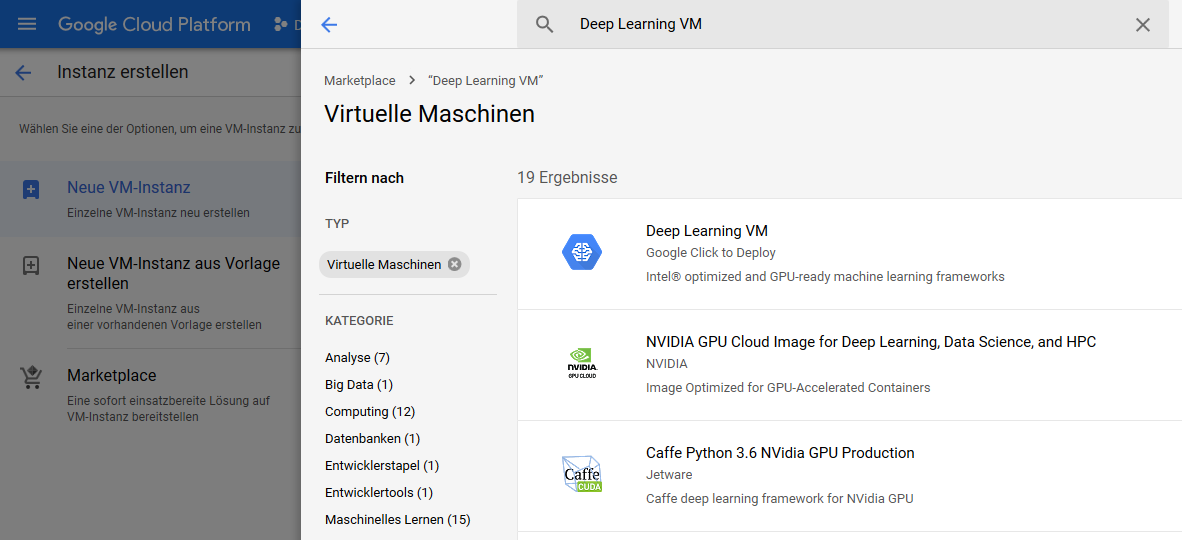
\includegraphics[width=\textwidth]{img/marketplaceSearch}}
	\caption{Searching for "Deep Learning VM"}
	\label{fig_marketplaceSearch}
\end{figure}
\noindent After you choose the virtual machine, you will be provided with some additional information. Choose ''start in compute engine'' as shown in picture \ref{fig_additionalInfo}.
\begin{figure}[H]
	\centerline{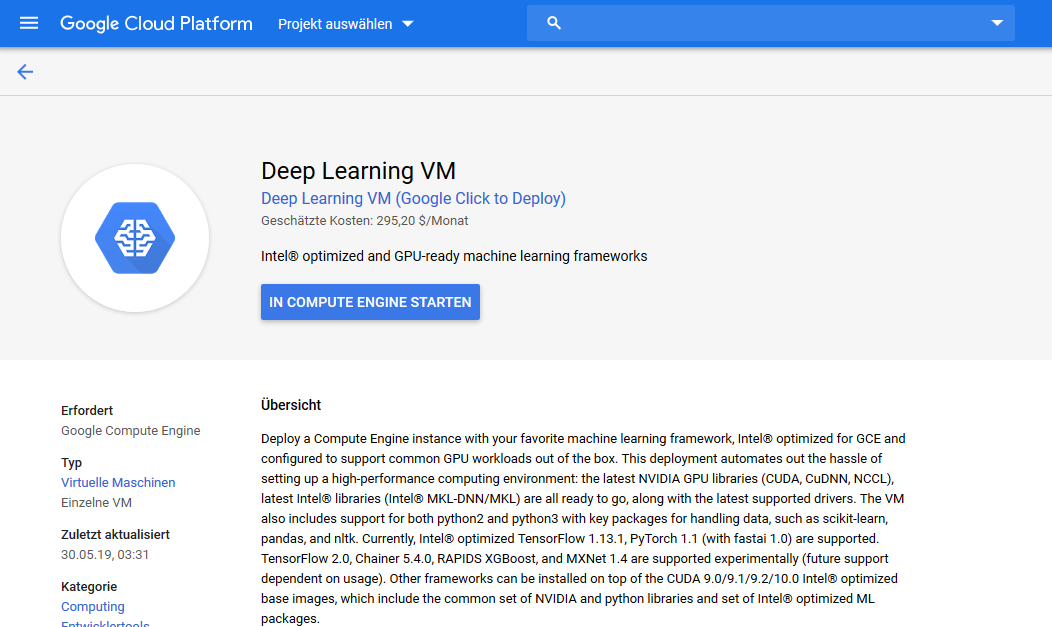
\includegraphics[width=\textwidth]{img/additionalInfo}}
	\caption{After selecting "Deep Learning VM"}
	\label{fig_additionalInfo}
\end{figure}
\subsubsection{Installing Additional Software}
After we successfully created our first virtual machine instance, we need to install some additional software on the virtual machine. This is possible through an administrator console, which can be opened by clicking the ''SSH'' button in the ''virtual machine instances'' sub-menu, as shown in picture \ref{fig_adminConsole}. The open console can be seen in picture \ref{fig_adminConsole2}.\\
\begin{figure}[H]
	\centerline{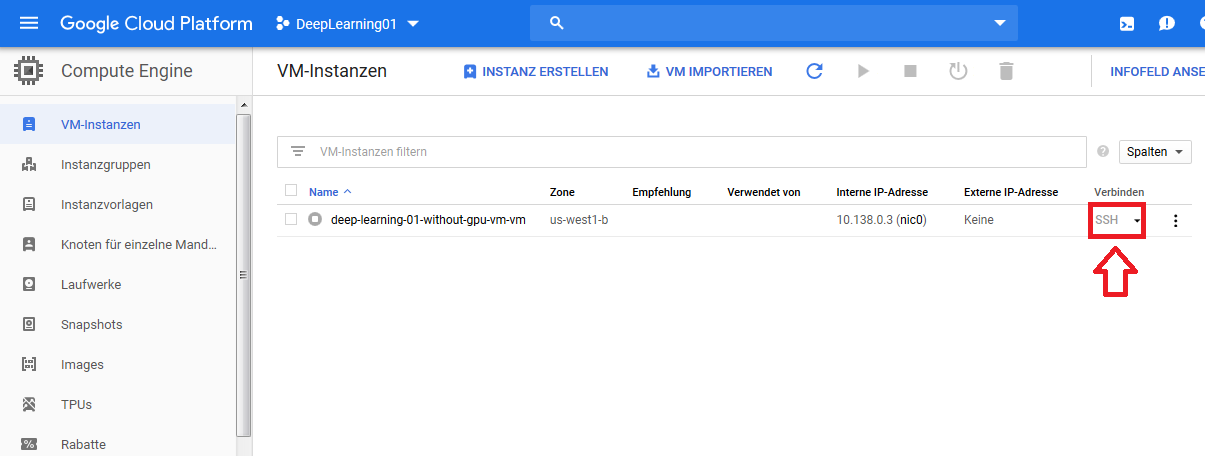
\includegraphics[width=\textwidth]{img/adminConsole}}
	\caption{The ''SSH'' button}
	\label{fig_adminConsole}
\end{figure}
\begin{figure}[H]
	\centerline{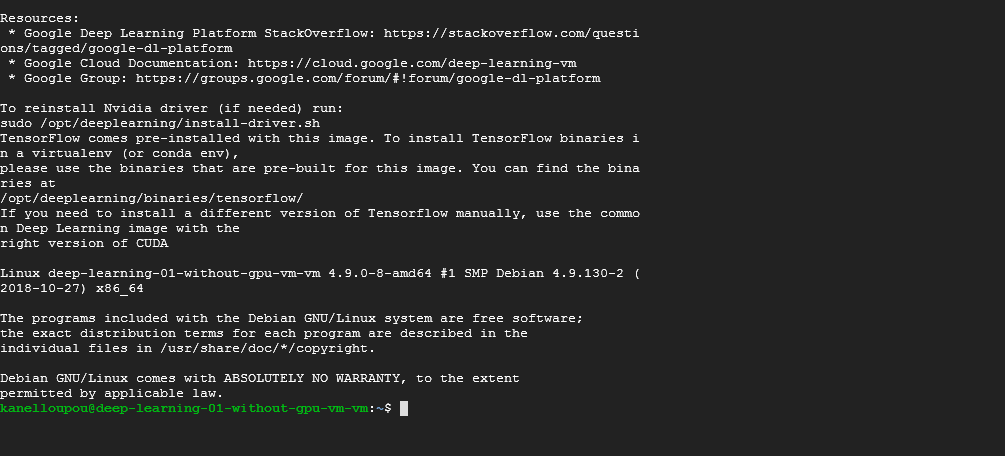
\includegraphics[width=\textwidth]{img/adminConsole2}}
	\caption{The administrator console}
	\label{fig_adminConsole2}
\end{figure}


\subsection{}

\end{document}
